\section{Dynamic response of QGP to electromagnetic fields}\label{chap:QCD}
\subsection{Plasma properties of QGP}

In this chapter, we discuss the application of the ultrarelativistic limit of the polarization tensor in Chapter \ref{chap:PlasmaSF} to the electromagnetic properties of quark-gluon plasma (QGP), as found in \cite{Grayson:2022asf}. QGP is an extreme state of matter composed of free quarks and gluons, which occurs in the aftermath of colliding nuclei in particle accelerators and existed a few microseconds after the big bang \cite{Letessier:2002ony}. 

The electromagnetic fields generated by colliding relativistic heavy ions in particle colliders are some of the largest in the known Universe, on the order of $ec|B| \approx m_\pi^2$, but exist for very short times $t_{\text{coll}}= 2 R/\gamma \sim 10^{-25}\,\textrm{s}$ due to the Lorentz contraction of the colliding nuclei. The magnetic field generated in these collisions is interesting due to its role in separating electric charge in the QGP through the chiral magnetic effect (CME) \cite{Kharzeev:2007jp}. The electric current generated by the CME could lead to a charge separation along magnetic field lines. If a magnetic field survives in QGP until the time of hadronization of the QGP, which we will refer to as the freeze-out time $t_f$, it could also lead to a difference in the global polarization of $\Lambda$ hyperons and antihyperons \cite{Muller:2018ibh}. Charge separation in the hadron was recently studied in \cite{STAR:2023jdd}. 

\begin{figure}[ht]
    \centering
    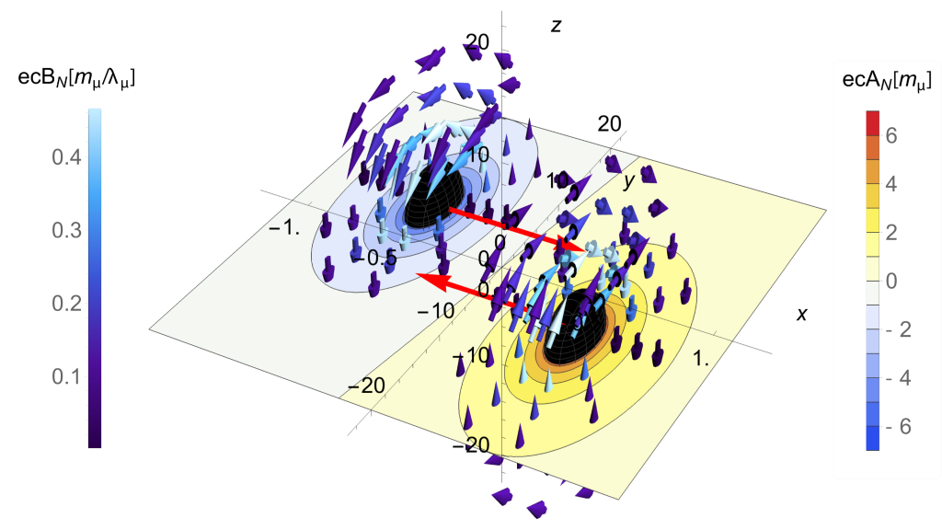
\includegraphics[width=0.85\linewidth]{plots/chap02QCD/Bfield.png}
    \caption{The vacuum magnetic field for two colliding lead Pb nuclei is shown for impact parameter $b=3R$ and $\gamma =37$. (At larger Lorentz factors, a graphical representation is difficult to visualize without scaling the fields with $\gamma$). The vector potential is plotted in the collision plane, and red arrows indicate the direction of the moving nuclei. This plot mainly shows the magnetic field distribution, which is Lorentz contracted along the direction of motion. The magnetic field lines circulate out of the collision plane perpendicular to the velocity, adding together at the collision center. \radapt{Grayson:2024okq}.}
    \label{fig:vacmag}
\end{figure}

The distribution of the vacuum magnetic field given by the Li\'enard-Wiechert fields is plotted in \reff{fig:vacmag}. This is the same magnetic field found by Lorentz boosting the Coulomb field of a nucleus at rest. We neglect the portion of the field that depends on acceleration since it is small for vacuum scattering of heavy nuclei, compared to the field that depends on velocity.

This magnetic field is treated as an external perturbation on the quark-gluon plasma, filling the overlap region between the two nuclei after they collide. For simplicity, the QGP is modeled as an infinite medium so that complications do not arise at the boundary. The temperature of QGP depends strongly on the collision energy of the nuclei. In \cite{Grayson:2022asf} we study Au+Au collisions at $\sqrt{s_{\text{NN}}}=200\,$GeV with QGP temperature $T=300$\,MeV.  After Heavy Ions collide, the conducting QGP medium generates long-range decaying tails or wakefields in the magnetic field that extend far beyond the collision time \cite{Tuchin:2010vs}. The conductivity of QGP determines the strength of these wakefields. We aim to model these fields in QGP using the formulation discussed in Chapter \ref{chap:PlasmaSF}.

\para{EM conductivity of quark-gluon plasma}
Past analytic calculations \cite{Tuchin:2010vs,Deng:2012pc,McLerran:2013hla,Tuchin:2013apa,Gursoy:2014aka,Li:2016tel,Roy:2015kma} solve Maxwell's equations in the presence of static electric conductivity 
\begin{equation}
   \sigma_0 = \frac{m_D^2}{3\kappa}\,,
\end{equation} 
in a  hydrodynamically evolving QGP. For a collisionless plasma $\kappa\rightarrow0$, the conductivity is infinite, and the medium behaves as a perfect conductor. This work introduces the frequency and wavevector dependence of the QGP analytically using the polarization tensor previously obtained in \cite{Formanek:2021blc}.

Numerical calculations \cite{Inghirami:2016iru,Inghirami:2019mkc} have incorporated the dynamical response of QGP by numerically solving the coupled magneto-hydrodynamic equations for a conducting quark-gluon plasma in the presence of the colliding nuclear charges. More recent calculations \cite{Yan:2021zjc,Wang:2021oqq} also incorporate the frequency and wave-vector dependence of QGP response to electromagnetic fields by solving the coupled Vlasov-Boltzmann--Maxwell equations\index{Vlasov-Boltzmann equation}  numerically.

\para{The Ultrarelativistic EM polarization tensor in QGP}\label{sec:linresp}
Here we review the ultra-relativistic polarization tensor, including damping, for the idealized case where the QGP is infinite, homogeneous, and stationary. This calculation differs from \cite{Formanek:2021blc} only in that we consider three quark species: up, down, and strange. We start with the Vlasov-Boltzmann equation for each quark flavor \req{eq:boltzmanncov} where we assume all quarks collide on a momentum-averaged time scale $\tau_{\text{rel}} = \kappa^{-1}$. The induced current $ j_{\mathrm{ind}}^\mu$ can be written in terms of the phase-space distribution of quarks and anti-quarks as
\begin{equation}\label{eq:current}
   j_{\mathrm{ind}}^\mu(x) = 2 N_c \int (dp)p^\mu \\ \times \sum_{u,d,s} q_f (f_{f}(x,p) - f_{\bar{f}}(x,p))=  4 N_Q e^2 \int (dp)p^\mu \delta f(x,p)\,,
\end{equation}
where  $N_c$ is the number of colors. We sum over the quark flavors with charges $q_f$, and in the final result, we replace $q_f \delta f = \delta f_f$. The result \req{eq:current} differs from that found in the case of an electron-positron plasma by the factor
\begin{equation}
N_Q \equiv N_c\sum_f (q_f/e)^2 = 2\,,
\end{equation}
for three light quark flavors ($u,d,s$).

In the ultrarelativistic limit, neglecting quark masses, one finds the polarization functions \cite{Formanek:2021blc}:
\begin{align}\label{eq:polfuncsUltra}
&\Pi_{\parallel}(\omega,|\boldsymbol{k}|) = m_D^2\frac{\omega^2}{\boldsymbol{k}^2}\left(1 - \frac{\omega \Lambda}{2|\boldsymbol{k}|-i\kappa \Lambda}\right)\,,\\
&\Pi_{\perp}(\omega,|\boldsymbol{k}|) = \frac{m_D^2\,\omega}{4 |\boldsymbol{k}|}\left( \Lambda \left(\frac{\omega'^2}{\boldsymbol{k}^2} - 1\right) - \frac{2\omega'}{ |\boldsymbol{k}|}\right)\,,
\end{align}
where $\Lambda(\omega,\boldsymbol{k})$ is defined as
\begin{align}\label{eq:definitions}
 \Lambda \equiv \ln \frac{\omega'+  |\boldsymbol{k}|}{\omega'- |\boldsymbol{k}|}\,, \quad \text{with} \quad \omega' = \omega+i\kappa\,.
\end{align}
The parallel and transverse polarization functions have the same form as in \cite{Formanek:2021blc} except for an overall factor $N_Q$  as found in \cite{Kapusta:1992fm,Grayson:2022asf}:
\begin{equation}\label{eq:DebyemQCD}
    {m_D}^2_{(\text{EM})} = \sum_{u,d,s} q^2_f T^2 \frac{N_c}{3} = N_Q\frac{e^2T^2}{3} \equiv C_{\text{em}}T^2\,,
\end{equation}
where $C_{\text{em}} =  2e^2/3$. In the following, we will use $m_D$ as short-hand notation for the electromagnetic screening mass since we do not discuss color screening here.
The transverse conductivity $\sigma_{\perp}$, which controls the response of the plasma to magnetic fields, is related to the imaginary part of the transverse polarization function as in \req{eq:sigmaperp}

\para{QCD Damping rate in QGP}
The strength of the plasma response to an external magnetic field depends on the quark damping rate $\kappa$ and the electromagnetic screening mass $m_D$. The scale of the collisional quark damping $\kappa$ is much larger than the electromagnetic Debye mass $m_D$ and electromagnetic damping $\kappa_{\text{EM}}$ because it depends on the strong coupling constant $\alpha_s$, not the electromagnetic coupling $\alpha$.

In \cite{Grayson:2022asf}, we use the first-order electromagnetic Debye mass \req{eq:DebyemQCD} to estimate the electromagnetic screening mass $m_D$. The collision rate $\kappa$ is related to the inverse of the mean-free time of quarks in QGP. We adopt a value for $\kappa$ from \cite{Mrowczynski:1988xu} where the mean-free time is given by the product of the parton density in the QGP and the quark-parton transport cross-section, leading to the expression 
\begin{equation}\label{eq:kappadef}
    \kappa(T) = \frac{10}{17\pi} (9 N_f +16) \zeta(3) \alpha_s^2 \ln\left(\frac{1}{\alpha_s}\right) T\,,
\end{equation}

\begin{figure}[ht]
    \centering
    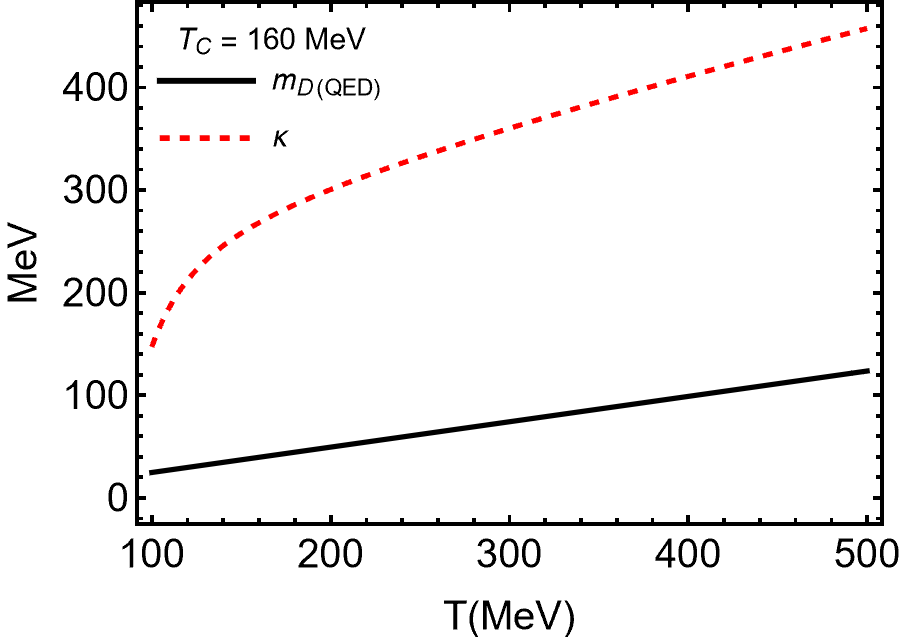
\includegraphics[width=0.85\linewidth]{plots/chap02QCD/kappaDEBYE.png}
    \caption{Plot of the electromagnetic Debye mass and the QCD dampening rate $\kappa$ as a function of temperature. At temperature $T=300\,$MeV used here, $\kappa = 4.86\, m_D$. \cccite{Grayson:2022asf}}
    \label{fig:kappaDebye}
\end{figure}

where $N_f$ is the number of flavors, $\zeta(x)$ denotes the Riemann zeta function, and $\alpha_s(T)$ is the running QCD coupling.  We model the running of the QCD coupling constant as a function of temperature in the range $T<5T_c$ using a fit provided in \cite{Letessier:2002ony}:
\begin{equation}\label{eq:alphas}
    \alpha_s(T) \approx \frac{\alpha_s(T_c)}{1+C \ln(T/T_c)}\,,
\end{equation}
where $C=0.760 \pm 0.002$. For the QCD (pseudo-)critical temperature we use $T_c = 160\,$MeV. The QED Debye mass is compared to $\kappa(T)$ in Fig.~\ref{fig:kappaDebye}. 
This is plotted along with the electromagnetic Debye mass in \reff{fig:kappaDebye}. We can expect the electromagnetic response of QGP response to be over-damped since $\kappa> \frac{2}{\sqrt{3} m_D}$ giving a plasma frequency \req{eq:plasmafreq} which is imaginary over the range of temperatures relevant for QGP.


\begin{figure}[ht]
    \centering
    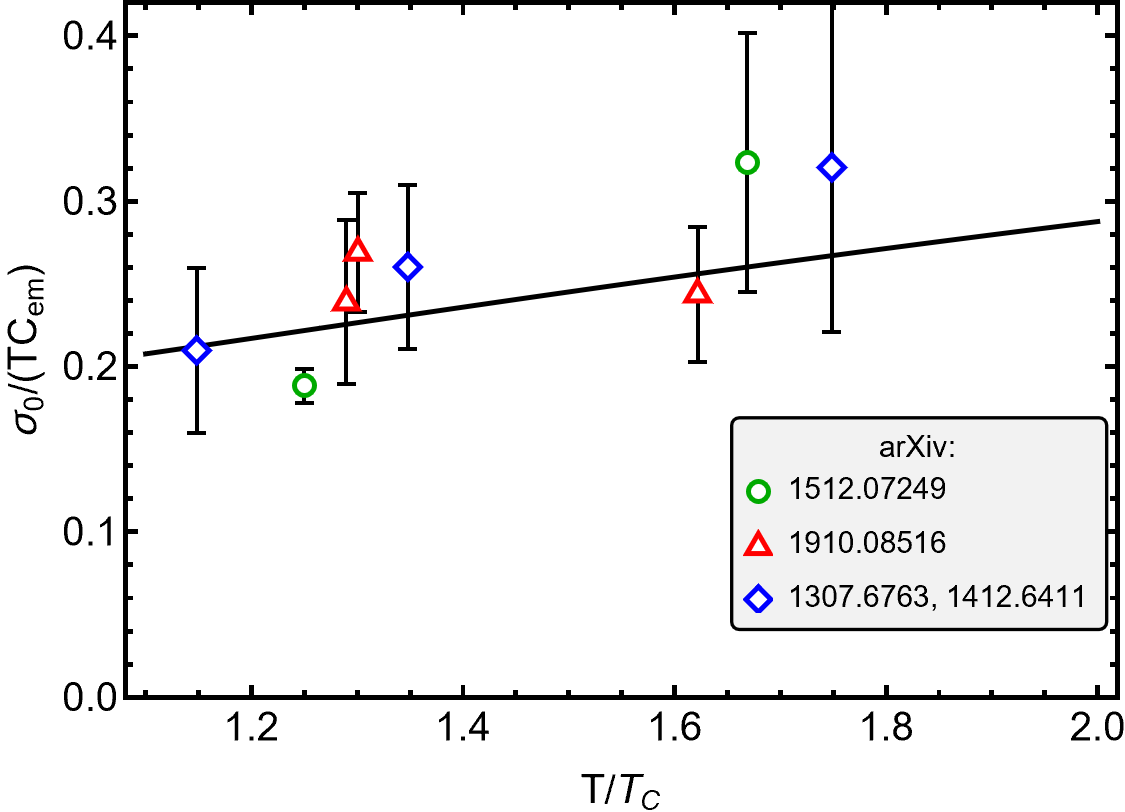
\includegraphics[width=0.85\linewidth]{plots/chap02QCD/condcomp.png}
    \caption{The black line shows the static conductivity $\sigma_0$ as a function of temperature predicted by \req{eq:condstat}, which is compared to lattice results adapted from \cite{Aarts:2020dda} for $T>T_c$. The factor of $C_{\text{em}}$, defined in \req{eq:DebyemQCD}, normalizes the conductivity by the charge of the plasma constituents, such that results using different numbers of dynamical quark flavors can be compared. We indicate each set of points by its arXiv reference: blue diamonds \cite{Amato:2013naa,Aarts:2014nba}, green circles \cite{Brandt:2015aqk}, and red triangles \cite{Astrakhantsev:2019zkr}. \radapt{Grayson:2024okq}.}
    \label{fig:lattice comp}
\end{figure}

We can then use the Debye mass \req{eq:DebyemQCD} and the damping rate \req{eq:kappadef} to calculate the static conductivity \req{eq:condstat}, shown as a black line in \reff{fig:lattice comp}, which we then compare to Lattice calculations of the conductivity in QGP.

These lattice-QCD results \cite{Amato:2013naa,Aarts:2014nba,Brandt:2015aqk,Astrakhantsev:2019zkr} are scaled with temperature $T$ to remove the linear temperature dependence. We also scale the conductivity with $C_{\text{em}}$, as defined in \req{eq:DebyemQCD}, such that computations with different numbers of flavors can be compared. One can see that the conductivity value predicted by \req{eq:kappadef}, plotted in Fig.~\ref{fig:lattice comp} as a black line, lies well within the lattice-QCD results. We will use the value predicted by \reff{fig:lattice comp}, $\sigma = 5.01\,$MeV at $T=300\,$GeV, in the next section to compute the screened heavy ion fields in QGP.

%%%%%%%%%%%%%%%%%%%
\label{sec:Maxwell2}
\para{Magnetic field in QGP during a nuclear collision}
Assuming that the QGP is an infinite homogeneous and stationary medium near equilibrium, we can solve Maxwell's equations for the self-consistent fields as in Section~\ref{sec:Maxwell}. Then the magnetic field is given by Fourier transforming the momentum space expressions given in \reqs{eq:aperp}{eq:ftfields} to position space
\begin{equation}\label{eq:magorgin}
   \boldsymbol{B}(t, z) = \int \frac{d^4k}{(2\pi)^4}  e^{-i\omega t+ik_z z}
 \frac{\mu_0 i \boldsymbol{k} \times\ft{j}_{\perp \text{ext}}(\omega, \boldsymbol{k})}{\boldsymbol{k}^2 - \omega^2 - \mu_0 \Pi_{\perp}(\omega, \boldsymbol{k})}\,.
\end{equation}
We choose the collision center as the origin of our spatial coordinate system and align the spatial $z$-axis with the beam direction. Due to the symmetry of the colliding ions, the only nonzero component of the magnetic field along the $z$-axis points out of the collision plane ($x-y$ plane). In our coordinate system used in \cite{Grayson:2022asf}, this corresponds to the $y$-component of the magnetic field. 

For ease of calculation, we specify the external 4-current using two colliding Gaussians charge distributions normalized to the nuclear rms radius $R$ and charge $Z$:
\begin{equation}\label{eq:rhoext}
\rho_{\text{ext}\pm }(t,\boldsymbol{x}) = \frac{Zq\gamma}{\pi^{3/2}R^3}e^{-\frac{1}{R^2}(x\mp b/2)^2}e^{-\frac{1}{R^2}y^2}
\times e^{-\frac{\gamma^2}{R^2}(z\mp \beta t)^2}\,,
\end{equation}
where $\gamma$ is the Lorentz factor, $\beta$ is the ratio of the ion speed to the speed of light, respectively, and $b$ is the impact parameter of the collision. The plus and minus signs indicate motion in the $\pm \hat{z}$-direction (beam-axis). This charge distribution corresponds to the vector current
\begin{equation}\label{eq:jext}
\boldsymbol{j}_{\text{ext}\pm}(t, \boldsymbol{x}) = \pm \beta \hatv{z} \rho_{\text{ext}\pm}(t, \boldsymbol{x})\,.
\end{equation}
Further details of the external charge distribution for two colliding nuclei are presented in Appendix B. of \cite{Grayson:2022asf}.

The numerical result for the position-space magnetic field found by Fourier transforming \req{eq:magorgin} using the full transverse polarization function \req{eq:polfuncsUltra} is shown as a red dashed line in Fig.~\ref{fig:bfcomp} and compared with various models of conductivity. These other models and their connections to published works are discussed in detail in \cite{Grayson:2022asf}.

\phantom{Phantom text}
\begin{figure}%[ht]
\centering              
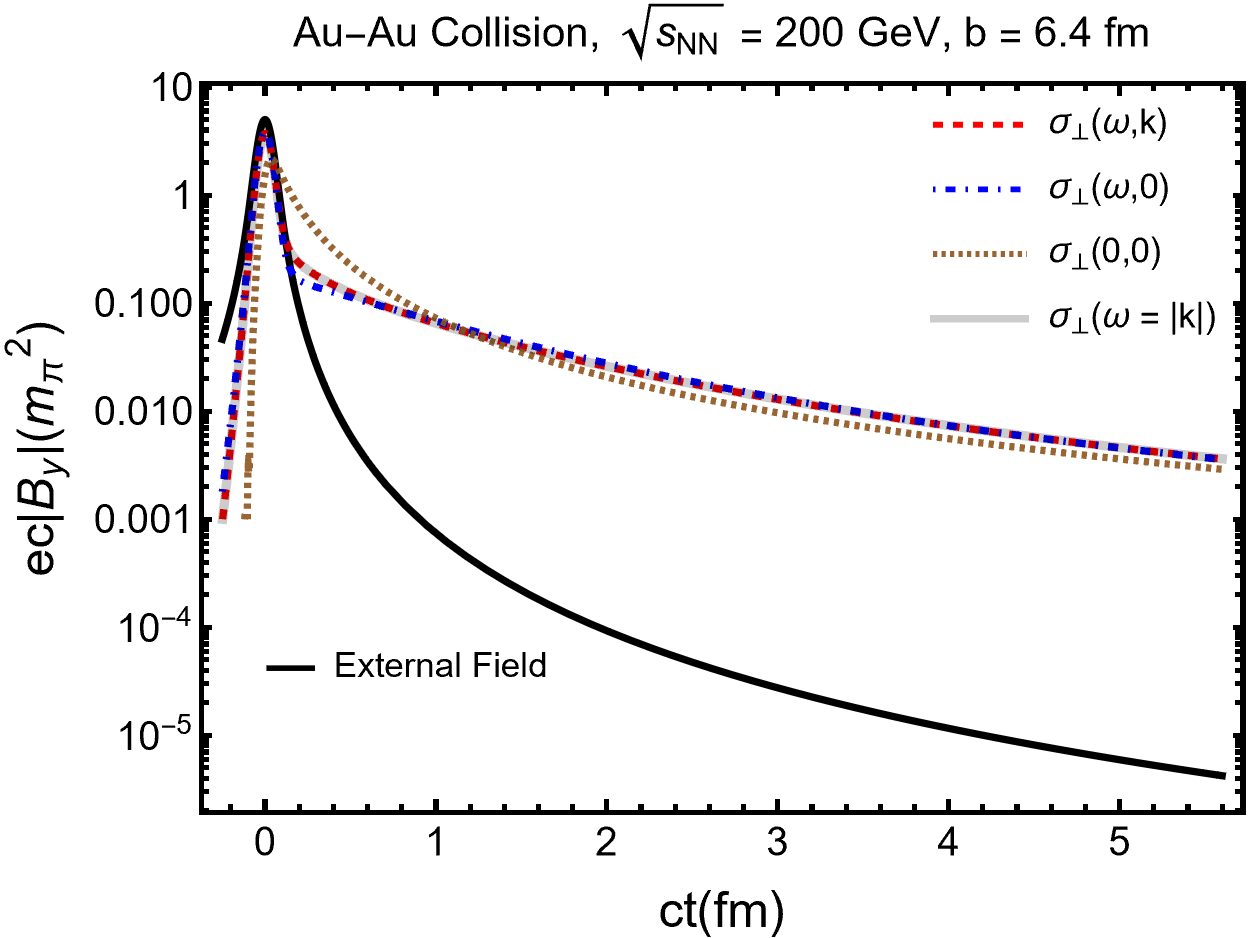
\includegraphics[width=0.75\linewidth]{plots/chap02QCD/bf100.png}\\
%}
\hspace{0.05\linewidth}
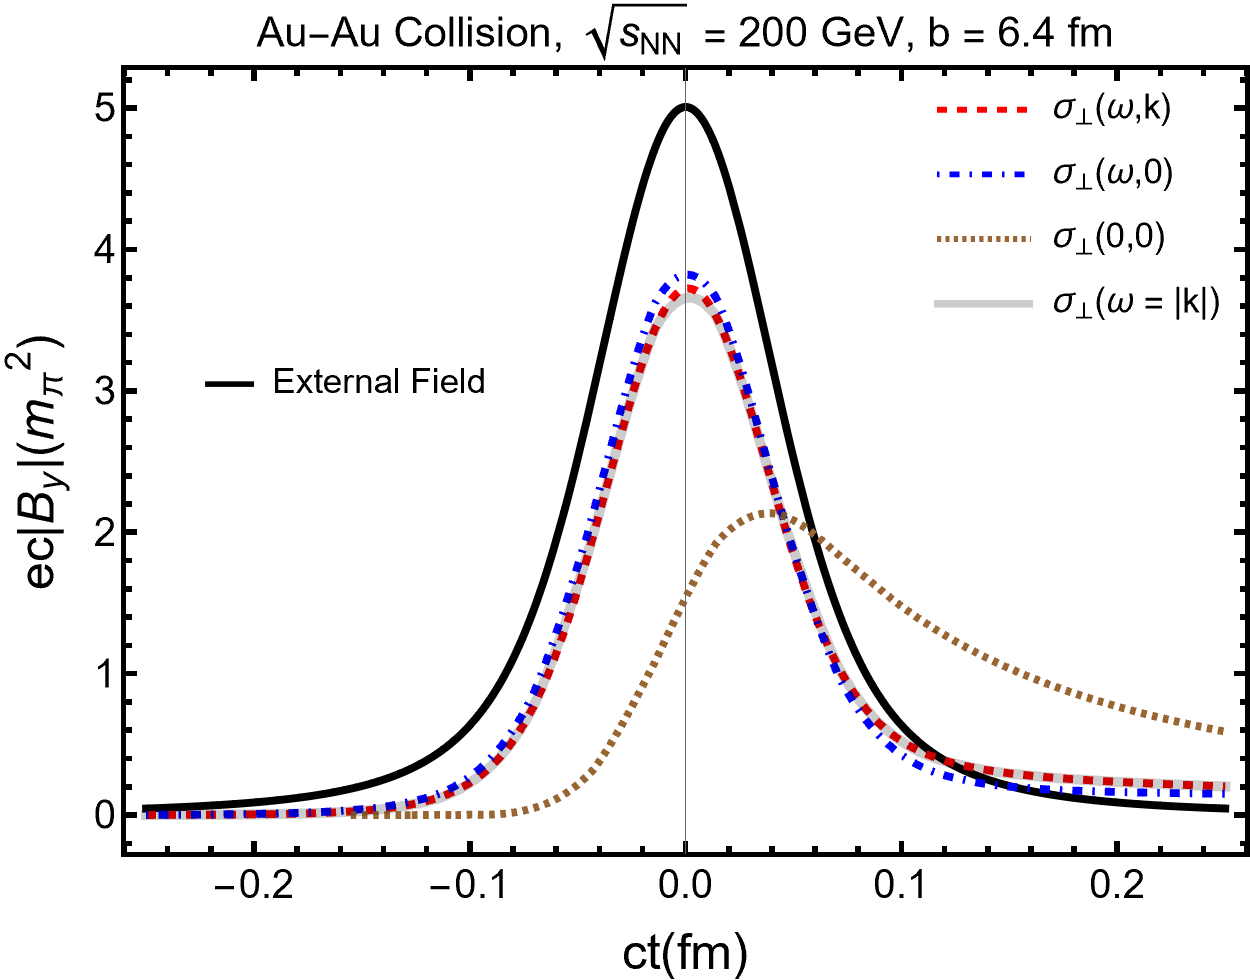
\includegraphics[width=0.75\linewidth]{plots/chap02QCD/bf100lin.png}
%}
\caption{The magnetic field at the collision center as a function of time, with $T = 300$\,MeV for Au-Au collisions ($Z=79$) at $\sqrt{s_\text{NN}} = 200$\,GeV and impact parameter $b = 6.4\,$fm. The left panel shows the magnetic field on a semi-logarithmic scale up to $ct = 5$\,fm. The right panel shows the early-time magnetic field on a linear scale. At the chosen temperature, the electromagnetic Debye mass is $m_D = 74\,$MeV, and the quark damping rate is $\kappa = 4.86\,m_D$. This gives a static conductivity of $\sigma_0 = 5.01\,$MeV. Comparing the different approximations, we see they all have similar asymptotic behavior. Only the Drude conductivity, the light-cone limit of the conductivity, and the full conductivity $\sigma_\perp(\omega,\boldsymbol{k})$ describe the field at early times. Note that the plasma is considered homogeneous and stationary here. In a more realistic situation, the field would become screened only after the QGP is formed in the collision. \cccite{Grayson:2022asf}\label{fig:bfcomp}}
\end{figure}

One of the important results of this paper was that the fields of the ions, traveling near the speed of light, probe the polarization tensor along the light cone. The transverse conductivity on the light cone is
\begin{equation}\label{eq:lightcone}
    \sigma_\perp (\omega = |\boldsymbol{k}|)  =  i \frac{m_D^2}{4 \omega}\left( \frac{\kappa^2}{\omega^2} \xi \ln\xi +\frac{i\kappa}{\omega}\left(\xi+1\right)\right)\,,
\end{equation}
where $\xi$ is defined as
\begin{equation}\label{eq:xidef}
    \xi \equiv 1- 2i \frac{\omega}{\kappa}\,.
\end{equation}
The light-cone conductivity simplifies the calculation of plasma response since it only depends on a single variable ($\omega = |\boldsymbol{k}|$). One can see that \req{eq:lightcone} shown as an opaque grey line traces out the full numerical solution \req{eq:magorgin} shown as a dashed red line. The light-cone conductivity accurately models the magnetic field in QGP since the ions traveling near the light's speed only sample the polarization tensor on the light-cone. One subject of future research is to use the light-cone conductivity to attain analytical formulas for electromagnetic fields in position space in light-cone coordinates.


The simplest method to calculate the late-time magnetic field of colliding nuclei is to assume a static conductivity \cite{Tuchin:2013apa}. In this case, the magnetic field in Fourier space has the form
\begin{equation}\label{eq:bstat}
    \ft{B}(\omega,\boldsymbol{k}) = \frac{ \mu_0 i\boldsymbol{k} \times \ft{j}_{\perp \text{ext}}}{\boldsymbol{k}^2 - \omega^2 - i\omega\sigma_0}\,,
\end{equation}
which is Fourier transformed using contour integration in the appendix of \cite{Grayson:2022asf} to
\begin{equation}\label{eq:banalyticapp}
   B_y(t) = -\mu_0 \frac{ Zq \beta }{(2\pi)} \frac{ b\sigma_0}{4t^2} e^{\frac{-b^2 \sigma_0}{16 t}}\,.
\end{equation}
Looking at the left panel of Fig.~\ref{fig:bfcomp}, the static conductivity initially overestimates the magnetic field after the external field begins to disappear since the effect of dynamic screening is not captured. Every model of the response function predicts similar values for the magnetic field approaching the freeze-out time $t_f \approx 5\,$fm/c \cite{Song:2007ux}. This is because the static conductivity determines the dependence of the magnetic field at times later than $t>1/\sigma \approx 59$\,fm/c after which damping of the initial magnetic field pulse is irrelevant. 

Alternatively, by assuming a point-like charge distribution $R\rightarrow0$ and approximating the magnetic field for $ 1/\sigma_0 > t\gg 1/\kappa$ one can derive the late-time magnetic field using the Drude conductivity \req{eq:drude}
\begin{equation}\label{eq:latetimeB}
   B_y(t) \approx  \mu_0 \frac{ Ze \beta b \kappa \omega_p }{8\pi}\bigg[ \frac{1- e^{-\kappa t}}{\kappa t} - e^{-\kappa t} \text{Ei}\left(t\kappa\right)\bigg]\,.
\end{equation}
This result has the advantage of accurately describing the late-time magnetic field $t>t_f$  at large $\gamma$ as shown in \reff{fig:bcolcomp}.

Both these results illustrate that the late-time magnetic field has a finite limit when $\gamma\rightarrow\infty$ as it depends only on $\beta$, but not on $\gamma$.
\begin{figure}
\centering
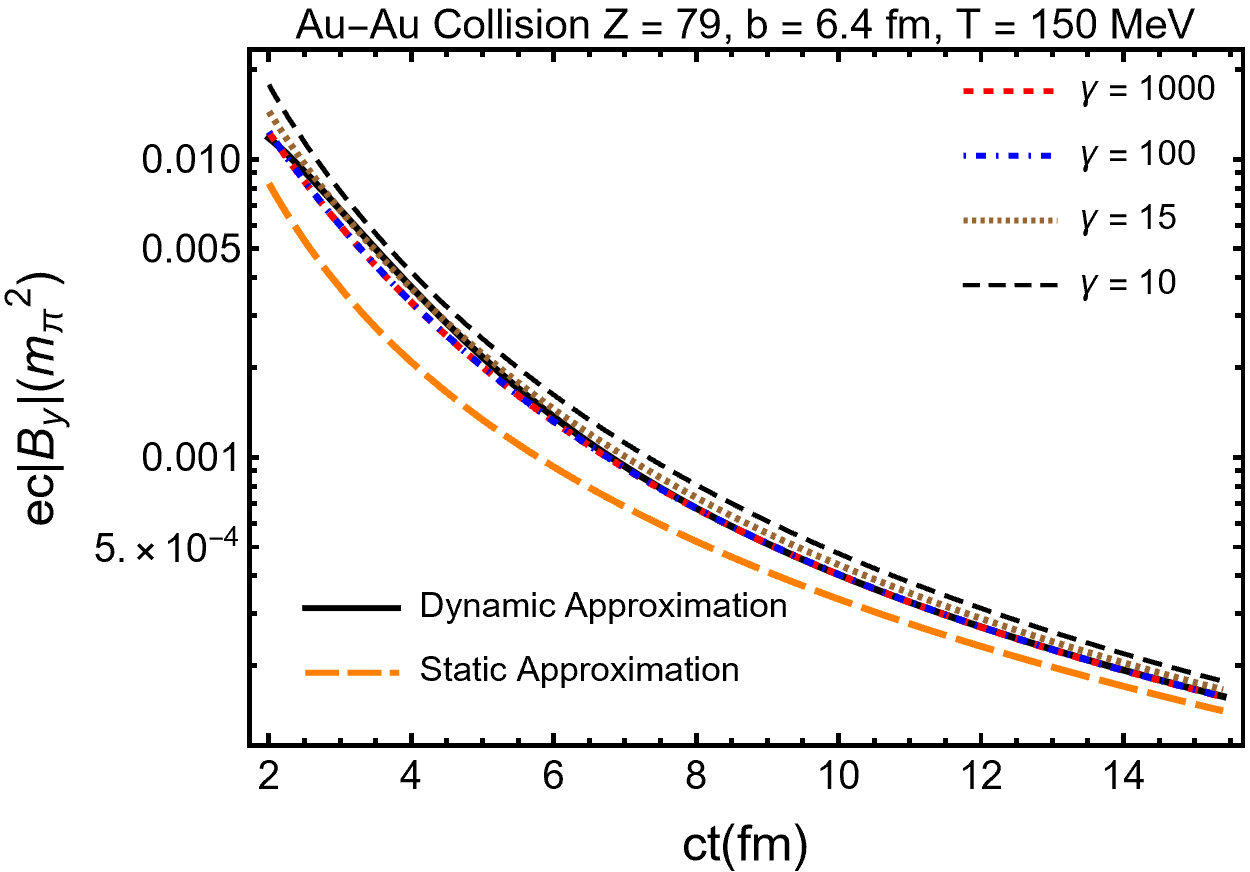
\includegraphics[width=0.85\linewidth]{plots/chap02QCD/bfgaamacomp.png}
    \caption{Plot of the freeze-out magnetic field for $T= 150$\,MeV. We expect that around this temperature QGP will hadronize into a mixed phase \cite{Letessier:1992xd}. The approximate late time solution \req{eq:banalyticapp} shown as an orange dashed line is compared to numerical calculations using the full polarization tensor \req{eq:magorgin} and to the late time analytic expansion \req{eq:latetimeB}. The approximate solution does not fully match the ultrarelativistic limit until times $t > t_{\sigma} \approx 59$\,fm/c. The magnetic field is independent of the beam energy over a wide range of $\gamma$ but begins to diverge slowly from the ultrarelativistic case at around $\gamma \leq 15$ for the time window shown in the figure. Lower beam energies result in a somewhat larger field at late times. \radapt{Grayson:2022asf}\label{fig:bcolcomp}}
\end{figure}
The approximation used to derive this solution holds for $\gamma\beta \gg \sqrt{ \kappa/\sigma_0} \approx 12$. In Fig.~\ref{fig:bcolcomp} we compare \req{eq:banalyticapp} to the full numerical result to explore its dependence on $\gamma$.  One can see that the static case \req{eq:banalyticapp} (black solid line) begins to diverge from the numerical solution, shown as dashed colored lines at around $\gamma \approx 15$.  In Fig.~\ref{fig:bcolcomp} one can see that the late-time magnetic field has a very soft dependence on collision energy. The time at which hadronization occurs $t_f$, which varies with collision energy, has a much stronger effect on the magnitude of the freeze-out field. Since the remnant magnetic field at hadronization does not depend strongly on the collision energy, an experimental measurement of the magnetic field at different collision energies could permit a determination of the electrical conductivity of the QGP or a determination of the freeze-out time of QGP if the conductivity is assumed to be known. 

As the QGP begins to hadronize at time $t_f$, one may expect hadrons to be statistically polarized with respect to the magnetic field. In \cite{Muller:2018ibh} the measured difference in global polarization of hyperons and antihyperons is used to give an upper bound on the magnetic field at QGP freeze-out, $B \sim 2.7\times 10^{-3}\,m_{\pi}^2$ for Au+Au collisions at $\sqrt{s_\text{NN}} = 200$\,GeV. Looking at Fig.~\ref{fig:bcolcomp} the magnetic field for $\gamma = 100$ at QGP freeze-out $t_f \approx 5 $\,fm/c is predicted to be $B \approx 1.2\times 10^{-3}\,m_{\pi}^2$, somewhat below this upper bound. Note that this assumes the polarization rapidly equilibrates in the plasma. It also neglects any interactions during the hadron gas phase of the collision. 

%%%%%%%%%%%%%%%
\subsection{Towards a more realistic QGP }\label{sec:ConclusionsQGP}
The work reviewed here calculates the magnetic field of two colliding nuclei in a stationary, homogeneous QGP using relativistic kinetic theory with collisional damping. Our first main finding in \cite{Grayson:2022asf} was that the response to the external magnetic field is controlled by the polarization function along the light-cone, $\Pi^\mu_\nu(\omega ,|\boldsymbol{k}|\approx\omega)$. This allowed us to derive an approximate analytic solution for the magnetic field that considers the dynamics of the medium's response. We also discussed how the late-time magnetic field at hadronization does not depend strongly on the collision energy. This gives the possibility that an experimental measurement of the magnetic field at different collision energies could permit a determination of the electrical conductivity of the QGP \cite{STAR:2023jdd}. We must also know how the freeze-out time depends on collision energy to make this measurement.

\para{The QGP medium}
This calculation can be improved in numerous ways. One of our main interests is to incorporate a finite size and a time-dependent onset in the QGP medium, which we describe here as infinite and homogenous. Boundary effects at the QGP surface are likely crucial for many collisions since the Debye sphere is not much smaller than the size of QGP, or similarly, the skin depth is probably large in comparison to the radius of QGP. Plasma skin effects could lead to novel electromagnetic phenomena at the QGP surface. We have begun some work on implementing an initial onset and formation time for QGP in the Vlasov-Boltzmann equation\index{Vlasov-Boltzmann equation} , effectively creating a boundary in time. This work should be extendable to studying plasma with a finite boundary in space which could be interesting with respect to the study of surface plasmons.

QGP is also not stationary; peripheral heavy ion collisions are one of the most highly rotational systems ever observed \cite{Csernai:2013bq,Deng:2016vhi,Jiang:2016woz,Becattini:2020pvq}. This is due to the huge angular momentum of the colliding system. This rotation can be incorporated into the equilibrium distribution \cite{Hakim:2011bk}, which creates a temperature that depends on radius \cite{Chernikov:1964edr} changing our description of the magnetic field.

In \cite{Grayson:2022asf} it would have been simple to use the adiabatic expansion of a relativistic ideal gas \cite{Bjorken:1982qr} to parameterize the temperature dependence as a function of time. To reduce the number of free parameters, we found the magnetic field at large times by simply assuming the plasma temperature was the freeze-out temperature \reff{fig:bcolcomp}.

Many enhancements can be made that require numerical solutions of the linear response equations, such improvements would include a realistic space-time dependence of the medium (formation and hydrodynamical evolution), nonzero net baryon density, quark thermal mass corrections \cite{Weldon:1982bn}, and viscous corrections to the unperturbed phase-space distribution used to calculate the polarization tensor.

\para{Electric field in QGP}
Of course, we could have also studied electric fields in QGP which are in the same order as the magnetic fields $e|E| \approx m_\pi^2$. These fields are of interest in strong field QED since they are far beyond the Schwinger limit $e|E| \approx m_e^2$. Preliminary QGP electric field calculations are shown in \reff{fig:efcomp}. In QGP, the transverse electric field $E_y$ is screened while the eclectic field is enhanced in the direction of motion. The electric field is also interesting since it could do a significant amount of work on the QGP possibly reheating it after its formation through ohmic heating. 

\phantom{Phantom text}
\begin{figure}%[ht]
\centering
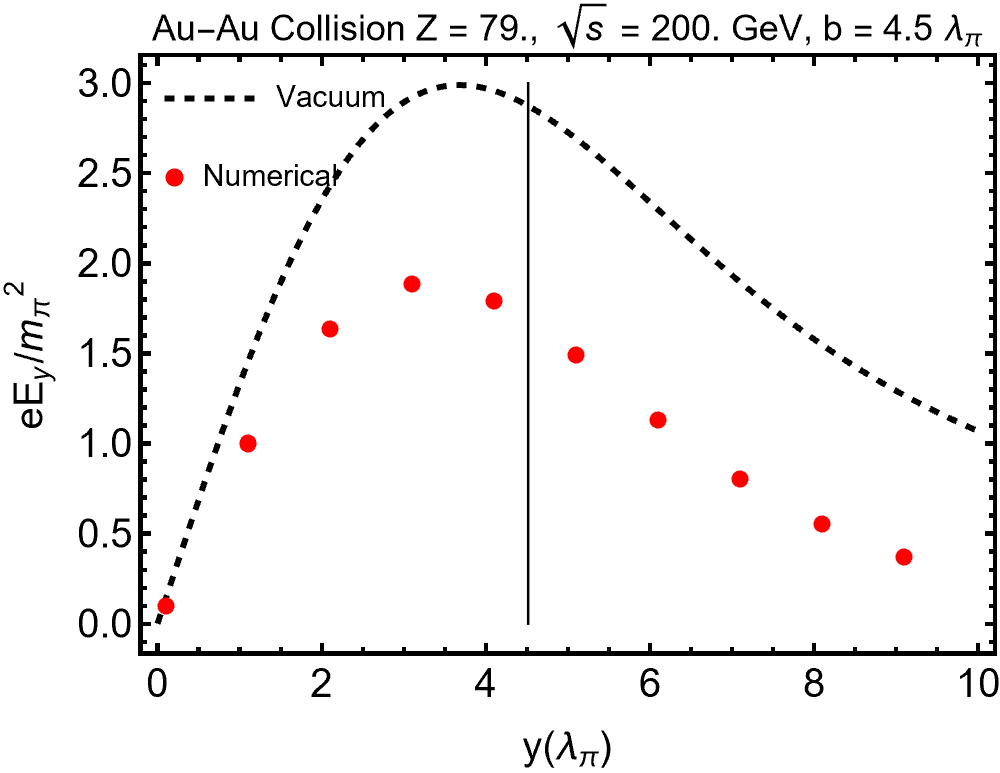
\includegraphics[width=0.75\linewidth]{plots/chap02QCD/Eyy.png}\\
%}
\hspace{0.05\linewidth}
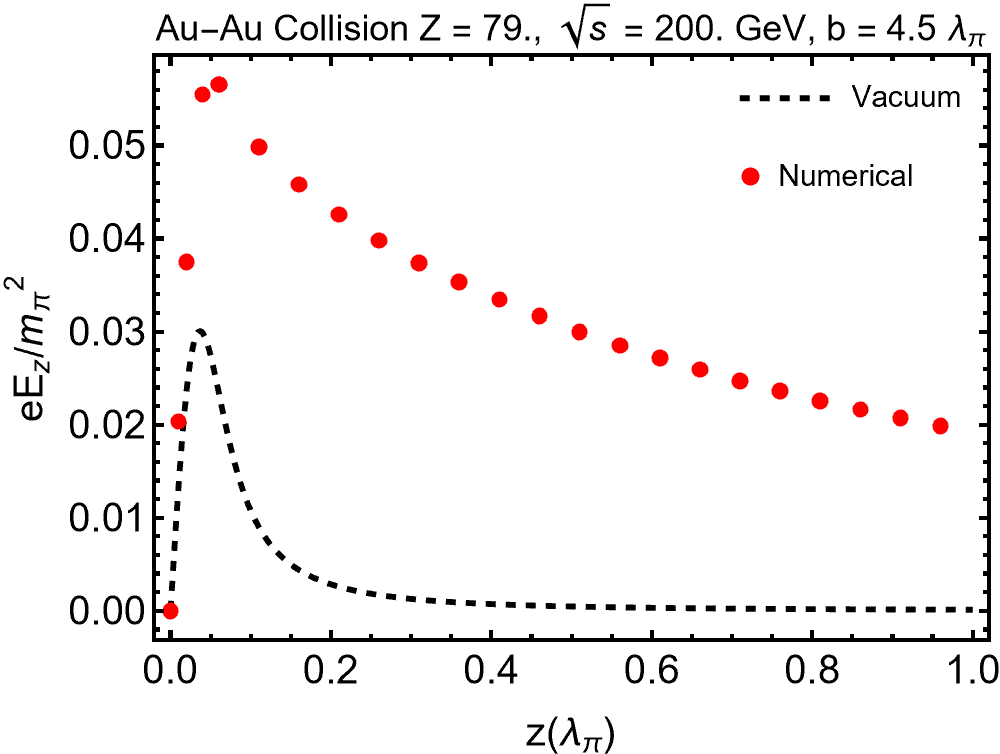
\includegraphics[width=0.75\linewidth]{plots/chap02QCD/Ezz.png}
%}
\caption{Plots comparing the electric field in vacuum, shown as a black dashed line, to the electric field in QGP shown as the red points. The left plot shows the transverse electric field screened by the plasma. The plot on the right shows the electric field in the direction of motion enhanced by the plasma. We choose $T = 300$\,MeV and $Z=79$, for Au-AU collisions at $\sqrt{s} = 200$\,GeV at an impact parameter of half nuclear overlap $b = 1 R = 6.4\,$fm. The vertical line in the left plot indicates $ y = R$, approximately the transverse size of QGP. \radapt{Grayson:2024okq}. \label{fig:efcomp}}
\end{figure}

Additionally, we were interested in studying the distribution of electric charge around relativistic heavy nuclei in QGP. This can be found by Fourier transforming \req{eq:indch} for the external charge distribution \req{eq:rhoext}. The induced charge density for a single traveling nucleus at low $\gamma$ is shown in \reff{fig:efcomp}. The external charge distribution increases with the Lorentz factor $\gamma$, but the total induced charge, which is the integral of the red dashed line, remains constant but trails behind further at larger velocities.

\phantom{Phantom text}
\begin{figure}%[ht]
\centering
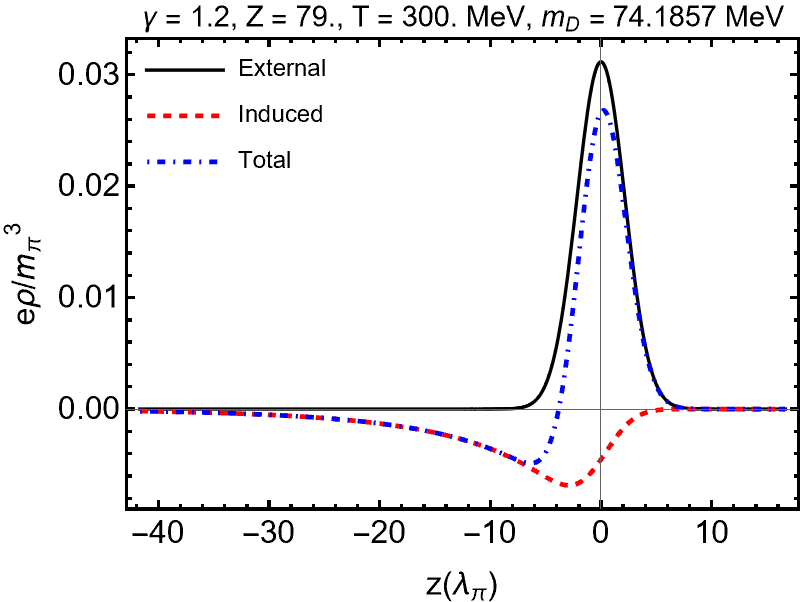
\includegraphics[width=0.75\linewidth]{plots/chap02QCD/indchg12.png}\\
%}
\hspace{0.05\linewidth}
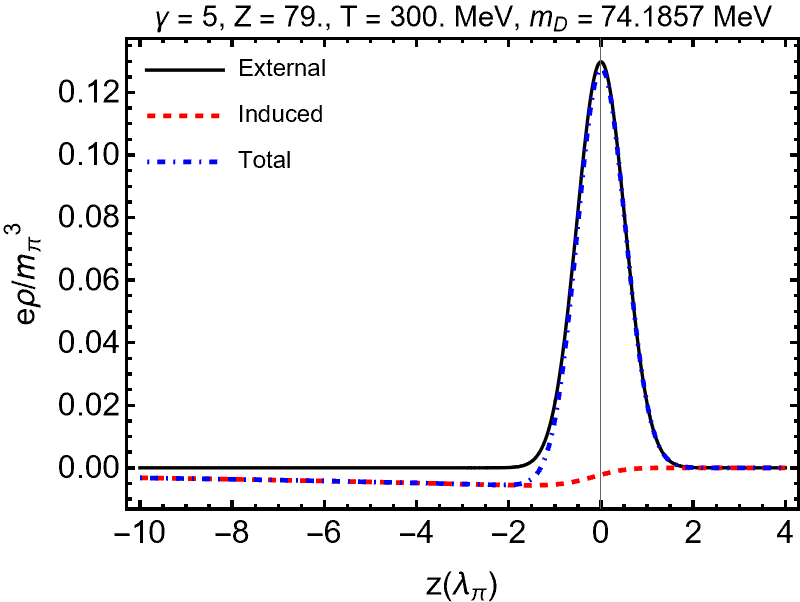
\includegraphics[width=0.75\linewidth]{plots/chap02QCD/indchg5.png}
%}
\caption{The external (black), induced (red dashed), and total charge density (blue dashed) for a single nucleus traveling in the $+\boldsymbol{\hat{z}}$ direction at $\gamma = 1.2$ on the left and $\gamma = 5$ on the right. The induced charge distribution trails behind the nuclei. The external charge density increases with $\gamma$. The induced charge distribution trails behind the nuclei more for larger $\gamma$ \label{fig:potcomp}. \radapt{Grayson:2024okq}.}
\end{figure}

As seen in \reff{fig:potcomp}, a wakefield of induced charge forms behind the traveling nucleus in QGP. In \reff{fig:chgwake}, we show a two-dimensional contour plot of the charged wake. The wakefield depicted in \reff{fig:chgwake} is damped at traverse distances instead of conical as in the collisionless case.
\begin{figure}[ht]
\centering
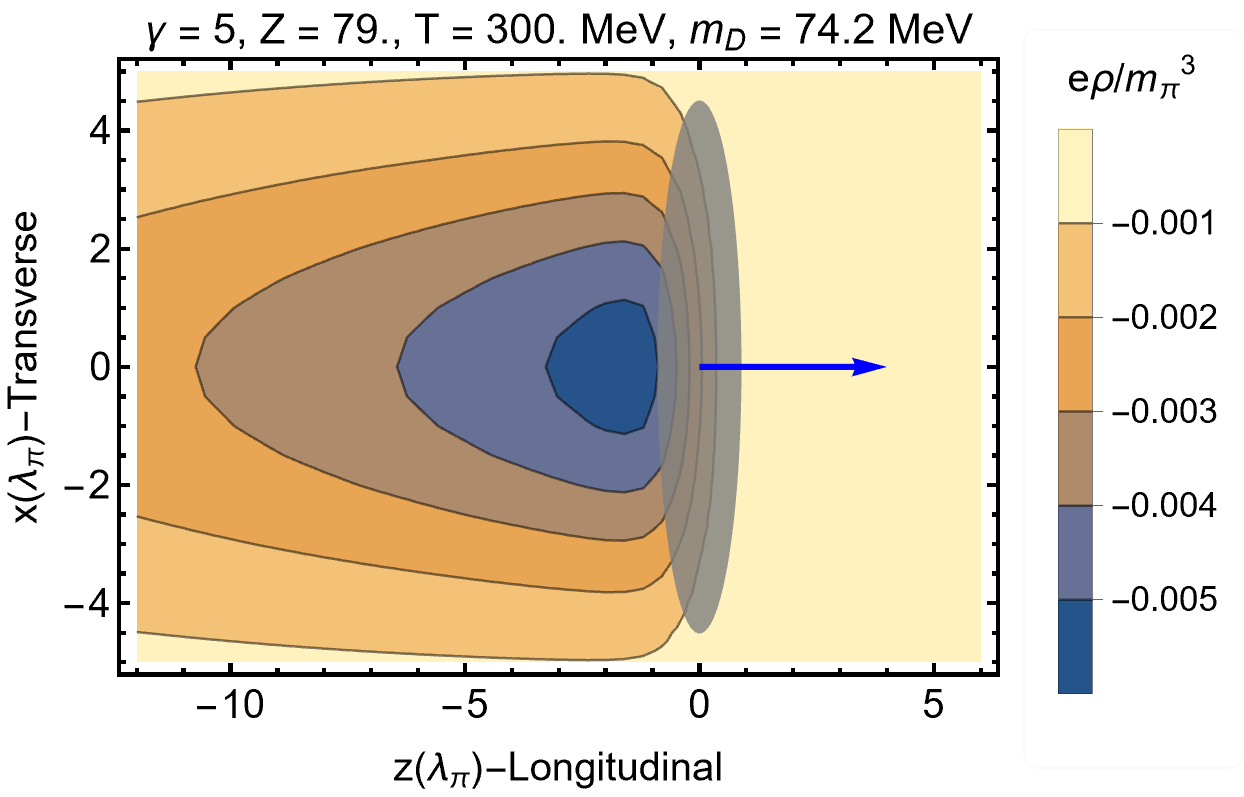
\includegraphics[width=0.85\linewidth]{plots/chap02QCD/chwake.png}
%}
\caption{2D plot of the wake field of a single traveling gold nucleus $\gamma = 5$ in QGP. The blue arrow indicates the direction of motion and the grey disk represents the Lorentz contracted nucleus. Lines of constant charge density are shown as contours. \radapt{Grayson:2024okq}.\label{fig:chgwake}}
\end{figure}


The Electromagnetic polarization tensor in QGP also has applicability in cosmology, where a QGP existed during the first $10~\mu$s of the early Universe. In the next chapter, we will study somewhat later times, a few seconds after the Big-Bang\index{Big-Bang}, when the universe was filled with electron-positron plasma\index{plasma!electron-positron}. In these situations, the assumption of homogeneity and stationary of the medium on the scale of the relevant parameters, $m_D$, and $\kappa$, is well justified.
